\begin{figure}[t]
    \centering
    \resizebox{0.62\textwidth}{!}{
    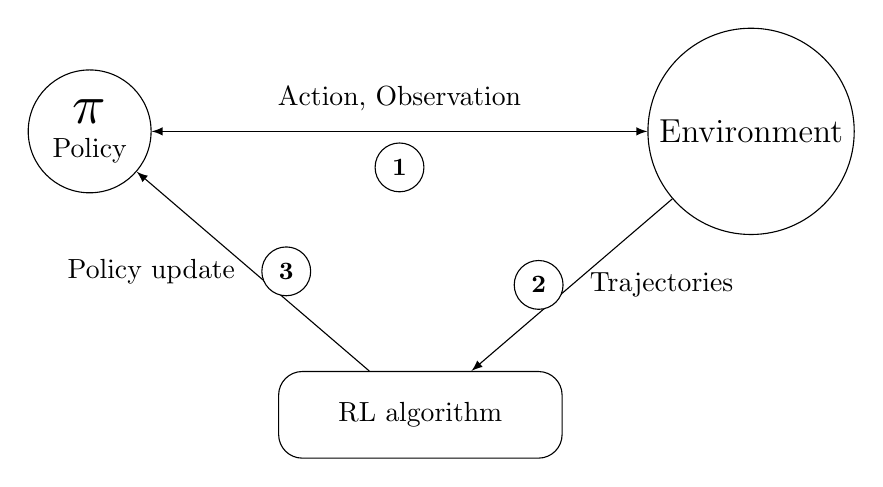
\begin{tikzpicture}[
        >=latex,
        stepmark/.style={draw, circle, fill=white, minimum size=0.62cm, inner sep=0pt, font=\bfseries\small},
    ]
        % Entities
        \node[draw, circle, align=center] (policy) at (-4.2, 0) {\scalebox{2}{$\pi$} \\ Policy};
        \node[draw, circle, align=center] (environment) at (4.2, 0) {\large Environment};
        \node[draw, rounded corners=0.3cm, minimum width=3.6cm, minimum height=1.1cm] (rl) at (0, -3.6) {RL algorithm};

        % 1. Agent--environment interaction
        \draw[<->] (policy) --
            node[above=4pt] {Action, Observation}
            node[below=4pt, stepmark] {1}
            (environment);

        % 2. Trajectories sent to the algorithm
        \draw[->] (environment) --
            node[left=3pt, stepmark] {2}
            node[right=3pt] {Trajectories}
            (rl);

        % 3. Policy update
        \draw[->] (rl) --
            node[right=3pt, stepmark] {3}
            node[left=3pt] {Policy update}
            (policy);
    \end{tikzpicture}
    }
    \caption{The three steps of a reinforcement learning iteration.}
    \label{fig:reinforcement_learning_loop}
\end{figure}
